
\begin{frame}{reliable flooding (picture)}

{\small Peterson and Davie, \textit{Computer Networks: A Systems Approach}, Figure 88}
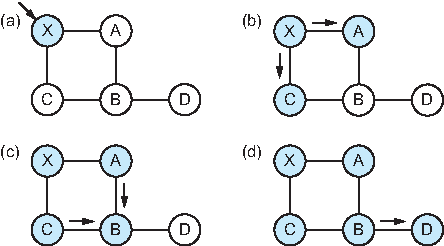
\includegraphics[width=0.8\textwidth]{../routing/sysapproach-fig88}
\end{frame}

\begin{frame}{missing from the picture}
    \begin{itemize}
    \item in picture: seems like each router directly connected to each other
    \item often we have multiple routers connected to local network
    \item can/will share link state packets by broadcasting on local network
    \end{itemize}
\end{frame}

\begin{frame}{reliable flooding in OSPF --- setup}
    \begin{itemize}
    \item for each subnetwork:
        \begin{itemize}
        \item choose a designated and backup router
        \item make sure backup becomes designated on failure
        \end{itemize}
    \item designated router will take care of propogating updates to everyone on network
    \item \ldots including waiting for acknowledgments, etc.
    \end{itemize}
\end{frame}

\begin{frame}{reliable flooding in OSPF}
    \begin{itemize}
    \item then, when receiving/generating link state packet:
    \item send to every designed+backup router of subnetwork that
        \begin{itemize}
        \item you are connected to, and
        \item you are not designated/backup router for, and
        \item you did not receive the packet from
        \end{itemize}
    \item send to every router on every subnetwork that
        \begin{itemize}
        \item you are designated router for
        \end{itemize}
    \item send = send + resend if no ACK
    \end{itemize}
\end{frame}

